% DIAPOSITIVA 10: El problema del histórico
\begin{frame}{Etapa 2: Costa Rica -- el problema del histórico}
  \begin{columns}[T]
    \begin{column}{0.54\textwidth}
      \textbf{Obstáculo técnico central:}
      \begin{itemize}
        \item Las plataformas solo muestran el \textbf{total acumulado hoy}
        \item Una publicación de oct.\ 2023 tiene hoy los likes de ago.\ 2026
        \item El tráfico póstumo (post-elección) \textbf{contamina} cualquier
              extracción retrospectiva estática
      \end{itemize}
      \vspace{0.3em}
      \textbf{Solución propuesta:}\\
      Modelar la función de crecimiento acumulado $F(t)$ de cada plataforma.
      Si conocemos la forma de la curva, podemos estimar cuántas interacciones
      tenía cualquier publicación en cualquier momento pasado.

      \vspace{0.3em}
      \textbf{Panel de calibración:} 1.ª vuelta Costa Rica, 1 feb.\ 2026
      \begin{itemize}
        \item 30 días de observación (15 antes, 15 después)
        \item 4 candidatos, 4 plataformas
        \item \num{1.922} publicaciones, \num{19.439} pares $(t, F)$
      \end{itemize}
    \end{column}
    \begin{column}{0.42\textwidth}
      \begin{block}{Intuición}
        Las reacciones llegan masivamente en las primeras horas y luego decaen.
        La curva es asimétrica: arranque explosivo, caída rápida, estabilización.
      \end{block}
      \vspace{0.5em}
      \textbf{Tres familias comparadas:}
      \begin{itemize}
        \item Exponencial simple
        \item Logística (inflexión simétrica)
        \item \kw{Weibull con offset}, ganadora
      \end{itemize}
    \end{column}
  \end{columns}
\end{frame}

% DIAPOSITIVA 11: Familia Weibull -- comparación
\begin{frame}{Etapa 2: Selección de la función de crecimiento}
  \begin{center}
  {\setlength{\tabcolsep}{3pt}
  \scriptsize
  \rowcolors{2}{tableBand}{white}
  \begin{tabular}{L{2.6cm} L{3.8cm} C{1.3cm} L{4.6cm}}
    \toprule
    \rowcolor{barBlue}
    {\color{white}\textbf{Modelo}} &
    {\color{white}\textbf{Ecuación}} &
    {\color{white}\textbf{$\bar{R}^2$}} &
    {\color{white}\textbf{Diagnóstico}} \\
    \midrule
    Exponencial simple &
      $F(t) = 1 - e^{-kt}$ &
      0,182 &
      Rígido; $\alpha \equiv 1$; subestima acumulación inicial \\
    Logístico &
      $F(t) = \dfrac{1}{1+e^{-k(t-t_0)}}$ &
      0,245 &
      Inflexión simétrica forzada; inadecuado para asimetría real \\
    \rowcolor{tableBand}
    \textbf{Weibull con offset} &
      $\bm{F(t) = 1 - e^{-k(t+t_0)^{\alpha}}}$ &
      \textbf{0,449} &
      Geometría flexible ($\alpha$); adelanto inicial ($t_0$); acotada en $[0,1]$ \\
    \bottomrule
  \end{tabular}}
  \end{center}

  \vspace{0.2em}
  \begin{columns}[T]
    \begin{column}{0.55\textwidth}
      \small\textbf{Interpretación correcta de los parámetros} \corr{[Corr.\ 1.6]}
      \begin{itemize}\small
        \item $k$: \textbf{tasa} de acumulación (no parámetro de escala clásico)
        \item $\alpha < 1$: acumulación desacelera (Facebook, Instagram, TikTok)
        \item $\alpha > 1$: tasa de acumulación \textbf{crece} (Twitter/X: $\alpha = 1{,}14$)
        \item $t_0 > 0$: \textbf{adelanto de origen}; $F(0) > 0$; modela interacciones
              previas al primer día de observación completo
      \end{itemize}
    \end{column}
    \begin{column}{0.41\textwidth}
      \begin{exampleblock}{Nota sobre $R^2$ moderado}
        \small El \num{66,8\%} de la varianza total es intra-publicación (ruido irreducible).
        El modelo captura la \textbf{forma global} de la curva, suficiente para la
        reconstrucción histórica.
      \end{exampleblock}
    \end{column}
  \end{columns}
\end{frame}

% DIAPOSITIVA 12: Parámetros calibrados
\addtocounter{framenumber}{1}

% DIAPOSITIVA nueva: Costa Rica -- ganadora vs. resto
\begin{frame}{Etapa 2: La ganadora es indistinguible del resto}
  \begin{center}
    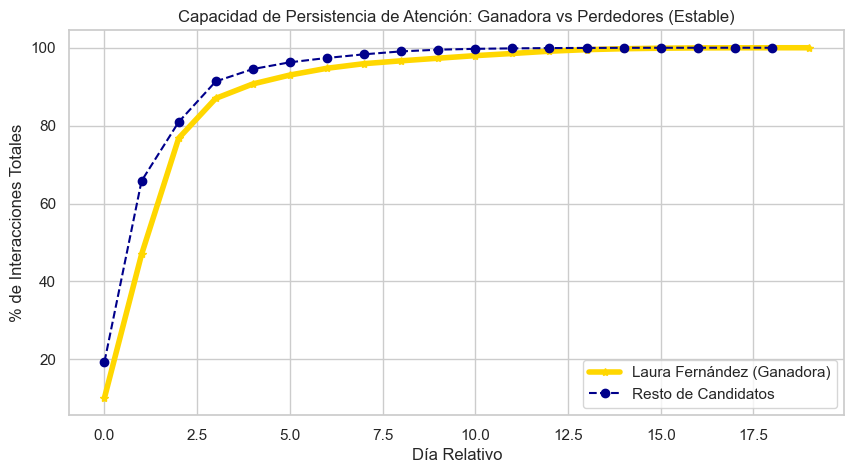
\includegraphics[width=0.80\textwidth]{img/costa_rica_ganadora.png}
  \end{center}
  {\footnotesize\color{subtleGray}\centering
    Laura Fernández (ganadora) vs.\ resto de candidatos.
    Sin diferencia estadísticamente significativa en ningún día del panel.
    El patrón de crecimiento es una propiedad de la \textbf{plataforma}, no del candidato.}
\end{frame}

% DIAPOSITIVA: Precisión proyectiva -- tabla MAPE
\addtocounter{framenumber}{1}

% DIAPOSITIVA nueva: MAPE convergencia + distribución de errores
\addtocounter{framenumber}{1}

% DIAPOSITIVA: Ajuste del restaurador por plataforma
\addtocounter{framenumber}{1}
